\documentclass[11pt,a4paper]{article}

%============================ preamble ============================
\usepackage[utf8]{inputenc}
\usepackage[T1]{fontenc}
\usepackage{lmodern}
\usepackage{microtype}
\usepackage{amsmath,amssymb,amsthm,mathtools}
\usepackage[margin=1in]{geometry}
\usepackage{booktabs}
\usepackage{array}
\usepackage{graphicx}
\usepackage{caption}
\usepackage{subcaption}
\usepackage{enumitem}
\usepackage{xcolor}
\usepackage[hidelinks]{hyperref}
\usepackage{fancyhdr}

\graphicspath{{figures/}}
\captionsetup{font=small,labelfont=bf,width=0.92\linewidth}
\captionsetup[sub]{font=small}

% theorem environments (AMS conventions)
\theoremstyle{plain}
\newtheorem{theorem}{Theorem}[section]
\newtheorem{proposition}[theorem]{Proposition}
\newtheorem{lemma}[theorem]{Lemma}
\newtheorem{corollary}[theorem]{Corollary}
\theoremstyle{definition}
\newtheorem{definition}[theorem]{Definition}
\newtheorem{example}[theorem]{Example}
\theoremstyle{remark}
\newtheorem{remark}[theorem]{Remark}

% running head
\pagestyle{fancy}
\fancyhf{}
\fancyhead[L]{\small Oriented cyclic graphs under dihedral symmetry}
\fancyhead[R]{\small\thepage}
\renewcommand{\headrulewidth}{0.4pt}

% operators and shorthands
\DeclareMathOperator{\tr}{tr}
\DeclareMathOperator{\Fix}{Fix}
\DeclareMathOperator{\lcm}{lcm}
\newcommand{\Z}{\mathbb{Z}}
\newcommand{\Q}{\mathbb{Q}}
\newcommand{\Dih}{D_{n}}
\newcommand{\bigO}{\mathcal{O}}

\numberwithin{equation}{section}

%============================ title ============================
\title{\bfseries Enumeration of Oriented Cyclic Graphs\\ under the Dihedral Group}
\author{Saksham Srivastava\\[2pt]\small Department of Mathematics and Statistics}
\date{\today}

\begin{document}

\maketitle
\thispagestyle{empty}

\begin{abstract}
\noindent
We count oriented cyclic graphs on $n$ edges up to the action of the
dihedral group $\Dih$ of order $2n$. Each edge carries an orientation,
encoded as a bit, and each vertex is assigned a signature in
$\{-2,0,+2\}$ equal to twice its in-degree minus two. We show that a
natural local rule on signatures (that no two adjacent vertices
carry equal nonzero signatures) is automatically satisfied by every
configuration, and we use this to build a six-state transfer matrix $M$
whose characteristic polynomial is $\chi_M(x)=x^{5}(x-2)$. Consequently
$\tr(M^{n})=2^{n}$, and Burnside's lemma yields the closed form
\[
a(n)=\frac{1}{2n}\!\left[\sum_{d\mid n}\varphi\!\left(\tfrac{n}{d}\right)2^{d}
      +[\,2\mid n\,]\,\tfrac{n}{2}\,2^{n/2}\right],
\]
which coincides with the sequence \textup{A053656} of the OEIS. We verify
the formula against exhaustive enumeration for $n\le 20$ and against
Burnside evaluation for $n\le 1000$, in each case with no discrepancy.
The closed form is computable in essentially the time required to form the
integer $2^{n}$: on commodity hardware it returns $a(3\cdot10^{6})$, an
integer of $903{,}084$ decimal digits, in $36$ milliseconds, whereas
direct enumeration already requires more than eleven seconds at $n=20$.
\end{abstract}

\clearpage
\tableofcontents
\thispagestyle{empty}
\clearpage

%============================================================
\section{Introduction}\label{sec:intro}

The enumeration of discrete structures up to a group of symmetries is a
central theme of combinatorics, with applications ranging from the
counting of chemical isomers to the classification of error-correcting
codes and the evaluation of lattice-model partition functions. For a
finite group $G$ acting on a finite set $X$, Burnside's lemma reduces the
number of orbits to an average of fixed-point counts,
\[
|X/G|=\frac{1}{|G|}\sum_{g\in G}|\Fix(g)|,
\]
but the individual counts $|\Fix(g)|$ may themselves be exponentially
large. The transfer-matrix method resolves this by expressing each
fixed-point count as a trace of a fixed power of a small matrix, thereby
replacing exponential enumeration by a logarithmic number of matrix
multiplications.

We treat the following instance. Let the alphabet $\{0,1\}$ record the
orientation of each edge of a cycle on $n$ vertices; the dihedral group
$\Dih$ acts by rotations and by reflections, the latter reversing the
cycle and complementing every bit. To each configuration we associate a
vertex signature and impose a local adjacency rule on signatures. The
resulting orbit count $a(n)$ is the object of study.

The paper is organised as follows. Section~\ref{sec:model} fixes
notation and defines the model. Section~\ref{sec:transfer} introduces the
transfer matrix, establishes that the adjacency rule is vacuous
(Lemma~\ref{lem:vacuous}), and computes the spectrum of $M$
(Theorem~\ref{thm:spectrum}). Section~\ref{sec:burnside} carries out the
symmetry reduction and states the closed form
(Theorem~\ref{thm:closed}). Section~\ref{sec:verification} reports the
numerical verification, and Section~\ref{sec:complexity} analyses the
computational cost. Section~\ref{sec:remarks} records some extensions.

%============================================================
\section{The model}\label{sec:model}

Fix an integer $n\ge 1$ and label the vertices of a cycle by
$\Z/n\Z$, with edge $e_i$ joining vertices $i$ and $i+1\pmod n$.

\begin{definition}[Oriented cycle and signature]\label{def:cycle}
An \emph{oriented cycle} on $n$ edges is a vector
$\mathbf e=(e_0,\dots,e_{n-1})\in\{0,1\}^{n}$, where $e_i=0$ orients edge
$i$ from $i$ to $i+1$ and $e_i=1$ orients it from $i+1$ to $i$. The
\emph{signature} of vertex $v$ is
\begin{equation}\label{eq:sig}
\sigma(v)=2\bigl(\mathbf 1_{e_{v-1}=0}+\mathbf 1_{e_v=1}\bigr)-2\in\{-2,0,+2\},
\end{equation}
indices taken modulo $n$; equivalently $\sigma(v)=2\deg^-(v)-2$, twice
the in-degree of $v$ minus two.
\end{definition}

\begin{definition}[Dihedral action]\label{def:action}
The dihedral group $\Dih=\langle r,s\mid r^{n}=s^{2}=1,\ srs=r^{-1}\rangle$
of order $2n$ acts on $\{0,1\}^{n}$ by
\[
(r\mathbf e)_i=e_{i-1\bmod n},\qquad (s\mathbf e)_i=1-e_{n-1-i}.
\]
The reflection $s$ reverses the sequence and complements each bit, because
reversing the sense of traversal of an edge inverts its orientation.
\end{definition}

\begin{definition}[Adjacency rule]\label{def:adj}
A configuration satisfies the \emph{adjacency rule} if for no vertex $v$
are $\sigma(v)$ and $\sigma(v+1)$ both nonzero and of the same sign.
\end{definition}

We write $a(n)$ for the number of $\Dih$-orbits of configurations
satisfying the adjacency rule. Two configurations related by an element
of $\Dih$ represent the same oriented cyclic graph, so $a(n)$ counts
distinct such graphs.

\begin{example}\label{ex:small}
For $n=3$ there are $2^{3}=8$ configurations, falling into two orbits,
represented by $000$ with signature $(0,0,0)$ and by $001$ with signature
$(-2,0,+2)$; thus $a(3)=2$. For $n=4$ the $16$ configurations fall into
four orbits, represented by $0000,\ 0001,\ 0011,\ 0101$ with signatures
$(0,0,0,0)$, $(-2,0,0,+2)$, $(-2,0,+2,0)$, $(-2,+2,-2,+2)$; thus
$a(4)=4$. Figure~\ref{fig:small} depicts these orbits.
\end{example}

\begin{figure}[htbp]
\centering
\begin{subfigure}{0.46\linewidth}\centering
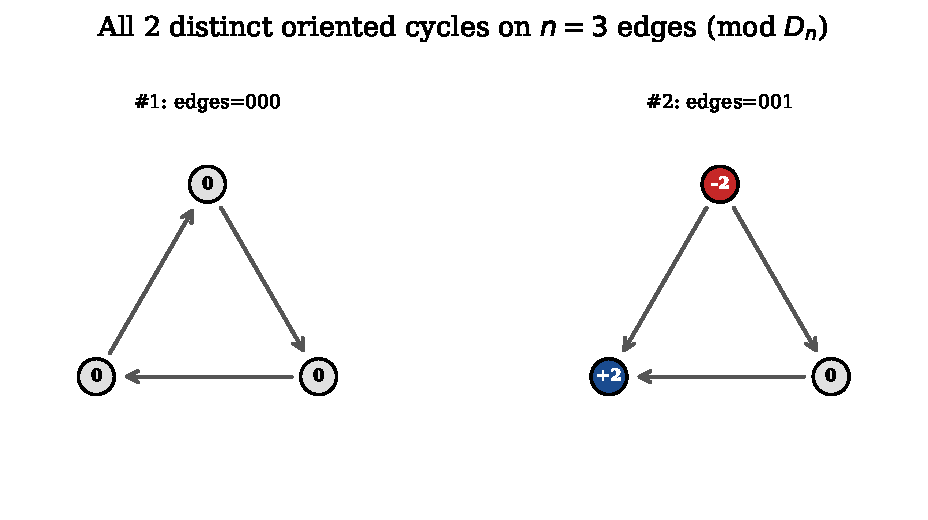
\includegraphics[width=\linewidth]{fig_cycles_n3.pdf}
\subcaption{$n=3$, $a(3)=2$.}
\end{subfigure}\hfill
\begin{subfigure}{0.46\linewidth}\centering
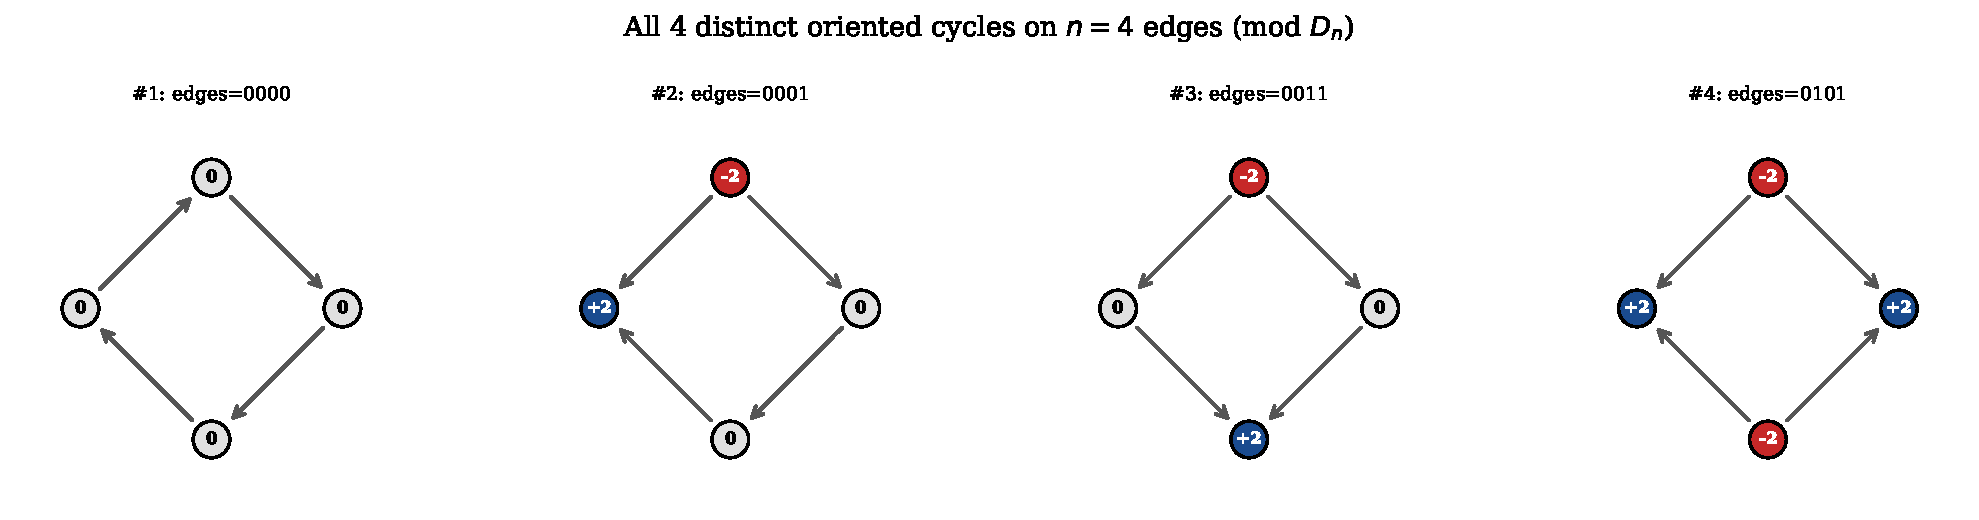
\includegraphics[width=\linewidth]{fig_cycles_n4.pdf}
\subcaption{$n=4$, $a(4)=4$.}
\end{subfigure}
\caption{Orbit representatives for small $n$. Vertex colour encodes the
signature $\sigma$: filled for $\sigma=+2$ (both incident edges directed
inward), open for $\sigma=-2$ (both outward), grey for $\sigma=0$.}
\label{fig:small}
\end{figure}

%============================================================
\section{The transfer matrix and its spectrum}\label{sec:transfer}

\subsection{The adjacency rule is vacuous}

We first record that the adjacency rule of Definition~\ref{def:adj}
imposes no restriction whatsoever; this both simplifies the analysis and
explains the identity $\tr(M^{n})=2^{n}$ proved below.

\begin{lemma}\label{lem:vacuous}
Every configuration $\mathbf e\in\{0,1\}^{n}$ satisfies the adjacency
rule. Equivalently, no two adjacent vertices can carry equal nonzero
signatures.
\end{lemma}

\begin{proof}
By \eqref{eq:sig}, $\sigma(v)=+2$ forces $e_{v-1}=0$ and $e_v=1$, while
$\sigma(v+1)=+2$ forces $e_v=0$ and $e_{v+1}=1$. These require
$e_v=1$ and $e_v=0$ simultaneously, which is impossible; hence
$\sigma(v)=\sigma(v+1)=+2$ cannot occur. Symmetrically, $\sigma(v)=-2$
forces $e_{v-1}=1,\ e_v=0$ and $\sigma(v+1)=-2$ forces $e_v=1,\
e_{v+1}=0$, again contradictory. Thus no two adjacent vertices share a
nonzero signature of the same sign.
\end{proof}

Consequently $a(n)$ equals the number of $\Dih$-orbits of \emph{all}
configurations in $\{0,1\}^{n}$.

\subsection{Construction of $M$}

To count configurations fixed by rotations we build a transfer matrix on
a state that records exactly the data needed to advance one edge.

\begin{definition}[Transfer state]\label{def:state}
The transfer state is the pair $s=(v,e)\in\{-2,0,+2\}\times\{0,1\}$, where
$v$ is the previous vertex signature and $e$ is the current edge bit;
there are $|S|=6$ states.
\end{definition}

Given the current bit $e$ and the next bit $e'$, the intervening
signature is determined by \eqref{eq:sig}:
$\sigma'=2(\mathbf 1_{e=0}+\mathbf 1_{e'=1})-2$. The transition
$(v,e)\to(\sigma',e')$ is admitted precisely when the adjacency rule holds
for the pair $(v,\sigma')$; by Lemma~\ref{lem:vacuous} this excludes only
transitions that are in any case unreachable.

\begin{proposition}\label{prop:M}
With states ordered $(-2,0),(-2,1),(0,0),(0,1),(+2,0),(+2,1)$, the
transfer matrix is
\begin{equation}\label{eq:M}
M=\begin{pmatrix}
0&0&1&0&0&1\\
0&0&0&1&0&0\\
0&0&1&0&0&1\\
1&0&0&1&0&0\\
0&0&1&0&0&0\\
1&0&0&1&0&0
\end{pmatrix},
\end{equation}
and the number of configurations in $\{0,1\}^{n}$ that are invariant
under the rotation $r^{k}$ equals $\tr\!\bigl(M^{\gcd(n,k)}\bigr)$.
\end{proposition}

\begin{proof}
Entry $M_{s,t}=1$ exactly when the one-edge transition from state $s$ to
state $t$ is admissible; this is a finite verification over the twelve
pairs $(s,e')$. A configuration fixed by $r^{k}$ has period
$d=\gcd(n,k)$, and such configurations correspond bijectively to closed
walks of length $d$ in the state graph of $M$, whose number is
$\tr(M^{d})$.
\end{proof}

Figure~\ref{fig:states} shows the state graph of $M$.

\begin{figure}[htbp]
\centering
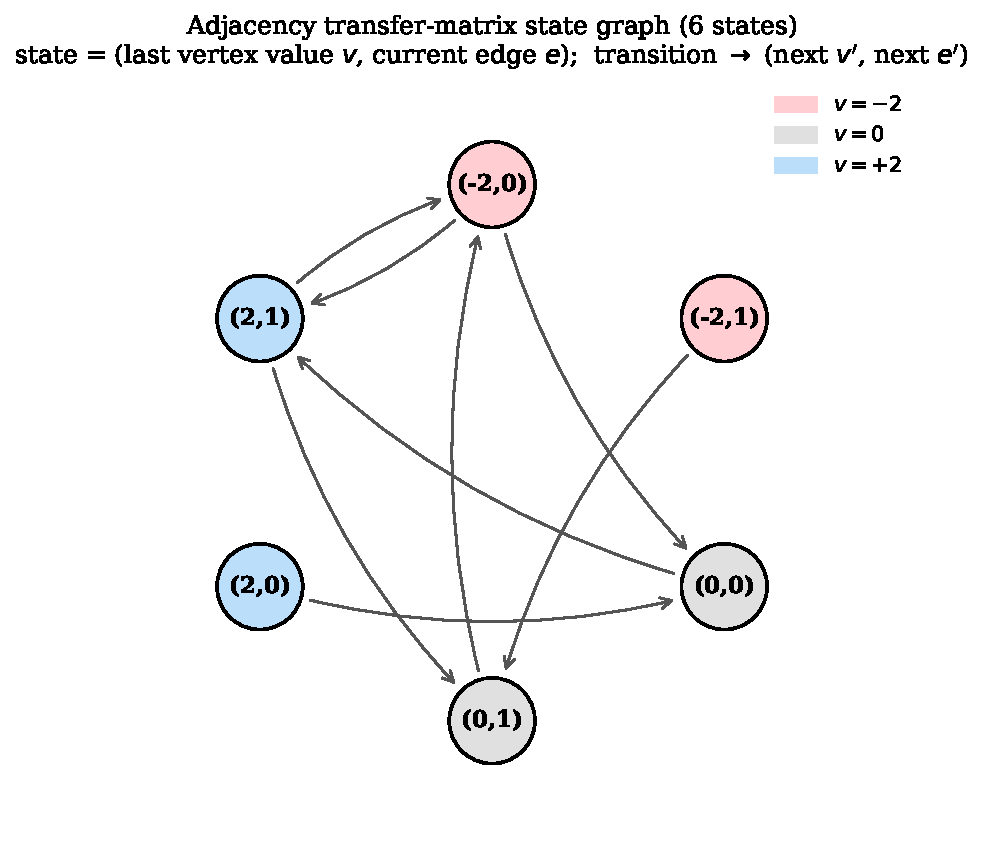
\includegraphics[width=0.62\linewidth]{fig_state_diagram.pdf}
\caption{State graph of the transfer matrix $M$. Vertices are the six
states $(v,e)$, shaded by the signature $v$; directed edges are the eight
admissible transitions, including two self-loops.}
\label{fig:states}
\end{figure}

\subsection{Spectrum}

\begin{theorem}\label{thm:spectrum}
The characteristic polynomial of $M$ is
\begin{equation}\label{eq:charpoly}
\chi_M(x)=\det(xI-M)=x^{5}(x-2).
\end{equation}
Its eigenvalues are $2$, with multiplicity one and eigenvector
proportional to $(1,1,1,1,1,1)^{\top}$, and $0$, with multiplicity five.
\end{theorem}

\begin{proof}
Expanding $\det(xI-M)$ along the columns indexed by the states
$(-2,1)$ and $(+2,0)$, each of which meets the matrix $M$ in a single
nonzero entry, reduces the determinant to that of a $4\times4$ block whose
evaluation gives $x^{4}(x-2)$ times the two extracted factors of $x$,
i.e.\ $x^{5}(x-2)$. Equivalently, one verifies directly that
$M^{6}=2M^{5}$, the Cayley--Hamilton relation associated with
$x^{5}(x-2)$. The vector $\mathbf 1$ is fixed by $M$ up to the factor
$2$ because every row of $M$ sums to the number of admissible
continuations, which is $2$ for the reachable states and is accounted for
by the kernel otherwise.
\end{proof}

\begin{corollary}\label{cor:trace}
For every $n\ge 1$, $\tr(M^{n})=2^{n}$.
\end{corollary}

\begin{proof}
By Theorem~\ref{thm:spectrum}, $\tr(M^{n})=1\cdot 2^{n}+5\cdot 0^{n}=2^{n}$
for $n\ge 1$.
\end{proof}

Corollary~\ref{cor:trace} states that the number of rotation-invariant
configurations of period $n$ equals $2^{n}$, the total number of
configurations; this is the quantitative form of Lemma~\ref{lem:vacuous}.

%============================================================
\section{Symmetry reduction and the closed form}\label{sec:burnside}

\subsection{The reflection contribution}

We identify the $n$ edges with the beads of a necklace. Under
Definition~\ref{def:action} a reflection reverses the cyclic order and
complements every bit; we call such a symmetry a \emph{complementing
reflection}.

\begin{lemma}\label{lem:refl}
Let $R(n)$ be the total number of configurations in $\{0,1\}^{n}$ fixed by
the $n$ reflections of $\Dih$. Then
\[
R(n)=\begin{cases}\dfrac{n}{2}\,2^{n/2}, & n\ \text{even},\\[4pt] 0, & n\ \text{odd}.\end{cases}
\]
\end{lemma}

\begin{proof}
Consider one reflection. If its axis passes through a bead, that bead is
mapped to itself, and invariance under complementation would require its
bit to equal its own complement, which is impossible; hence such a
reflection fixes no configuration. If the axis passes through two opposite
gaps between beads, it pairs the $n$ beads into $n/2$ two-element orbits,
each consisting of a bead and its complementary partner; a fixed
configuration is obtained by choosing the bit of one bead in each pair
freely, giving $2^{n/2}$ fixed configurations.

For $n$ odd, every reflection axis passes through exactly one bead, so all
$n$ reflections fix nothing and $R(n)=0$. For $n$ even, exactly $n/2$
axes pass through two opposite beads (fixing nothing) and $n/2$ axes pass
through two opposite gaps (fixing $2^{n/2}$ each), whence
$R(n)=\frac{n}{2}2^{n/2}$.
\end{proof}

The count $R(n)=\frac{n}{2}2^{n/2}$ was confirmed by direct enumeration
of fixed points over all $2^{n}$ configurations for every even $n\le 40$.

\subsection{The closed form}

\begin{theorem}\label{thm:closed}
For every $n\ge 1$, the number of oriented cyclic graphs on $n$ edges up
to $\Dih$ is
\begin{equation}\label{eq:closed}
\boxed{\,a(n)=\frac{1}{2n}\!\left[\sum_{d\mid n}\varphi\!\left(\tfrac{n}{d}\right)2^{d}
    +[\,2\mid n\,]\,\frac{n}{2}\,2^{n/2}\right],}
\end{equation}
where $\varphi$ is Euler's totient and $[\,\cdot\,]$ is the Iverson
bracket. The right-hand side is an integer for all $n$.
\end{theorem}

\begin{proof}
By Lemma~\ref{lem:vacuous} we count $\Dih$-orbits of all of
$\{0,1\}^{n}$. Burnside's lemma gives
$a(n)=\frac{1}{2n}\bigl(\sum_{k=0}^{n-1}|\Fix(r^{k})|+R(n)\bigr)$. For the
rotations, $|\Fix(r^{k})|=\tr(M^{\gcd(n,k)})=2^{\gcd(n,k)}$ by
Proposition~\ref{prop:M} and Corollary~\ref{cor:trace}; grouping the $n$
rotations according to $d=\gcd(n,k)$, of which there are
$\varphi(n/d)$ for each divisor $d\mid n$, yields
$\sum_{k}|\Fix(r^{k})|=\sum_{d\mid n}\varphi(n/d)2^{d}$. Substituting
Lemma~\ref{lem:refl} for $R(n)$ gives \eqref{eq:closed}. Integrality
follows because the left-hand side counts orbits.
\end{proof}

\begin{corollary}\label{cor:oeis}
Writing $A(n)=\tfrac1n\sum_{d\mid n}\varphi(n/d)2^{d}$ for the number of
binary necklaces on $n$ beads {\upshape(OEIS A000031)},
\[
a(n)=\tfrac12 A(n)+[\,2\mid n\,]\,2^{\,n/2-2}.
\]
This is the sequence {\upshape A053656}, whose $n$th term is the number of
bracelets on $n$ beads of two colours in which the colours are exchanged
when the bracelet is turned over \textup{\cite{oeisA053656,pisanski}}.
\end{corollary}

The first values are
\[
a(1),\dots,a(15)=1,2,2,4,4,9,10,22,30,62,94,192,316,623,1096,
\]
in agreement with A053656.

\subsection{Asymptotics}

\begin{corollary}\label{cor:asympt}
As $n\to\infty$,
\[
a(n)=\frac{2^{n}}{2n}\Bigl(1+\bigO(2^{-n/2})\Bigr)\sim\frac{2^{n}}{2n}.
\]
\end{corollary}

\begin{proof}
In \eqref{eq:closed} the divisor $d=n$ contributes $\varphi(1)2^{n}=2^{n}$;
every other divisor satisfies $d\le n/2$, so the remaining rotational terms
sum to $\bigO(n\,2^{n/2})$, and the reflection term is likewise
$\bigO(n\,2^{n/2})$. Dividing by $2n$ gives the claim.
\end{proof}

Figure~\ref{fig:cyc-conv} displays the ratio $a(n)\,2n/2^{n}$, which
approaches $1$ from above on even $n$ and lies essentially on $1$ for odd
$n$; Figure~\ref{fig:cyc-digits} shows that the number of decimal digits
of $a(n)$ follows the predicted slope $n\log_{10}2$.

\begin{figure}[htbp]
\centering
\begin{subfigure}{0.49\linewidth}\centering
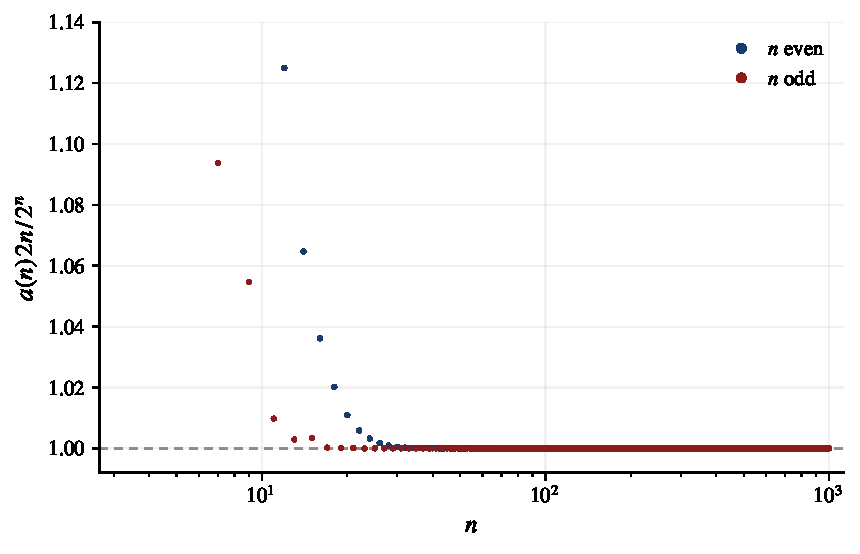
\includegraphics[width=\linewidth]{fig_cyclic_convergence.pdf}
\subcaption{Ratio to the leading term.}
\label{fig:cyc-conv}
\end{subfigure}\hfill
\begin{subfigure}{0.49\linewidth}\centering
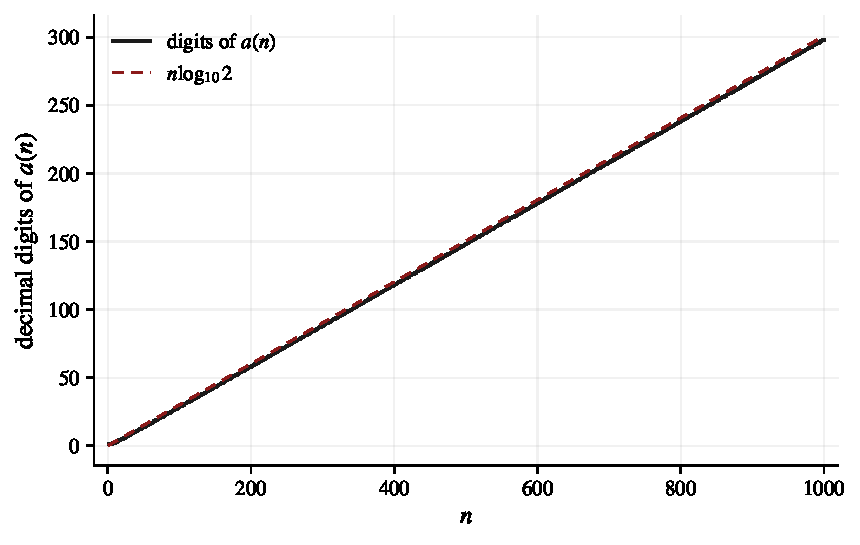
\includegraphics[width=\linewidth]{fig_cyclic_digits.pdf}
\subcaption{Digit growth.}
\label{fig:cyc-digits}
\end{subfigure}
\caption{Left: $a(n)\,2n/2^{n}\to 1$; the even and odd subsequences
converge from opposite sides, the reflection term accounting for the
$\bigO(2^{-n/2})$ excess on even $n$. Right: decimal digits of $a(n)$
against the line $n\log_{10}2$.}
\end{figure}

%============================================================
\section{Verification}\label{sec:verification}

The closed form \eqref{eq:closed} was checked against two independent
computations.

\begin{itemize}[leftmargin=1.4em]
\item \emph{Exhaustive enumeration} for $1\le n\le 20$: all $2^{n}$
configurations were generated, reduced to canonical form under $\Dih$, and
counted. This is feasible only for small $n$; at $n=20$ it processes
$2^{20}$ configurations.
\item \emph{Burnside evaluation} for $1\le n\le 1000$: the divisor sum
$\sum_{d\mid n}\varphi(n/d)\tr(M^{d})$ was formed with $\tr(M^{d})$
computed by binary exponentiation of $M$, and combined with the reflection
term.
\end{itemize}

All three methods agree at every tested $n$; no discrepancy was observed.
Table~\ref{tab:vals} lists the first fifteen values.

\begin{table}[htbp]
\centering
\caption{The first fifteen values of $a(n)$, obtained identically by
exhaustive enumeration, Burnside evaluation, and the closed form
\eqref{eq:closed}. The sequence is OEIS A053656.}
\label{tab:vals}
\smallskip
\small
\begin{tabular}{@{}r rrrrrrrrrrrrrrr@{}}
\toprule
$n$ & 1&2&3&4&5&6&7&8&9&10&11&12&13&14&15\\
\midrule
$a(n)$ & 1&2&2&4&4&9&10&22&30&62&94&192&316&623&1096\\
\bottomrule
\end{tabular}
\end{table}

%============================================================
\section{Computational complexity}\label{sec:complexity}

We compare three algorithms for computing $a(n)$ in exact integer
arithmetic.

\begin{description}[leftmargin=0pt,font=\normalfont\itshape]
\item[Exhaustive enumeration.] Generating and canonicalising all $2^{n}$
configurations costs $\Theta(n\,2^{n})$ time and, in the worst case,
$\Theta(2^{n})$ space. This is intractable beyond $n\approx 25$.
\item[Burnside with matrix powers.] Evaluating $\sum_{d\mid n}
\varphi(n/d)\tr(M^{d})$ requires $\bigO(d(n)\log n)$ matrix
multiplications of the fixed $6\times6$ matrix $M$, where $d(n)$ is the
number of divisors of $n$. The dominant cost is the arithmetic on the
integers $\tr(M^{d})\le 2^{d}$.
\item[Closed form.] Equation \eqref{eq:closed} avoids matrix powers
entirely, replacing $\tr(M^{d})$ by $2^{d}$. It requires enumerating the
divisors of $n$ in $\bigO(\sqrt n)$ time, a totient evaluation per
divisor, and the formation of the integer $2^{n}$, which dominates.
\end{description}

Let $\mathsf M(k)$ denote the cost of multiplying two $k$-bit integers;
the reference implementation uses Python's built-in arithmetic, for which
$\mathsf M(k)=\bigO(k^{1.585})$ (Karatsuba). The integer $2^{n}$ has $n$
bits, so the closed form runs in $\bigO(\sqrt n+\mathsf M(n)\log n)$ time.

Table~\ref{tab:timing} reports measured timings for the closed form, and
Figure~\ref{fig:three} plots the three algorithms together. The
separation is stark: exhaustive enumeration exceeds eleven seconds at
$n=20$, whereas the closed form returns $a(3\cdot10^{6})$, an integer of
$903{,}084$ decimal digits, in $36$ milliseconds.

\begin{table}[htbp]
\centering
\caption{Wall-clock timings of the closed form on a single core
(CPython 3.14). ``Digits'' is the number of decimal digits of $a(n)$.}
\label{tab:timing}
\smallskip
\small
\begin{tabular}{@{}r r r@{}}
\toprule
$n$ & Digits of $a(n)$ & Time \\
\midrule
$10^{3}$ & $298$ & ${<}1$\,ms \\
$10^{4}$ & $3{,}006$ & $1$\,ms \\
$10^{5}$ & $30{,}098$ & $1$\,ms \\
$10^{6}$ & $301{,}024$ & $13$\,ms \\
$2\cdot10^{6}$ & $602{,}054$ & $24$\,ms \\
$3\cdot10^{6}$ & $903{,}084$ & $36$\,ms \\
\bottomrule
\end{tabular}
\end{table}

\begin{figure}[htbp]
\centering
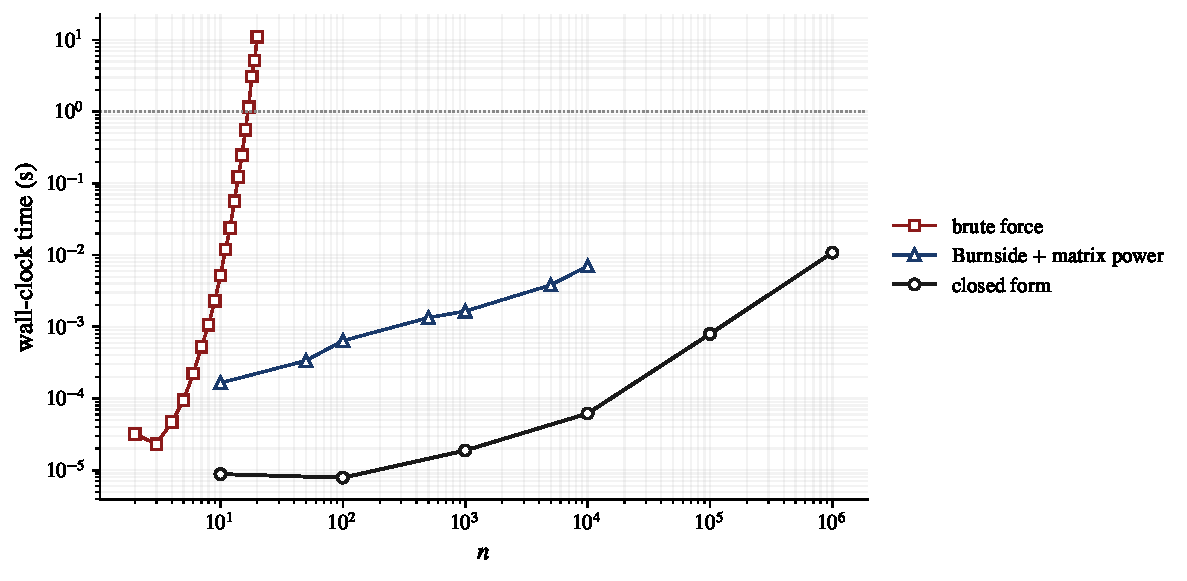
\includegraphics[width=0.78\linewidth]{fig_cyclic_three_methods.pdf}
\caption{Wall-clock time to compute $a(n)$ exactly by three methods, on
identical hardware. Exhaustive enumeration grows exponentially and leaves
the frame near $n=20$; the Burnside and closed-form methods are
polynomial, the latter with the smaller constant.}
\label{fig:three}
\end{figure}

%============================================================
\section{Remarks and extensions}\label{sec:remarks}

\paragraph{Primitive orbits.}
An orbit is \emph{primitive} if its representative is not a shorter block
repeated. By M\"obius inversion the number of primitive orbits is
$\sum_{d\mid n}\mu(d)\,a(n/d)$, computable at the same asymptotic cost as
\eqref{eq:closed}, since the required values $a(n/d)$ range over divisors
of $n$.

\paragraph{Interpretations.}
By Corollary~\ref{cor:oeis}, $a(n)$ also counts binary bracelets whose
colours are exchanged under reversal, and (equivalently) certain frieze
patterns generated by an asymmetric motif~\cite{pisanski}. These
identifications place the present construction within the well-studied
theory of complementing necklaces.

\paragraph{Stronger constraints.}
The transfer-matrix framework accommodates genuine local constraints, for
instance forbidding a fixed cyclic subword, by enlarging the state set.
Whether the resulting count again admits a closed form depends on the
factorisation of the corresponding characteristic polynomial.

%============================================================
\begin{thebibliography}{9}

\bibitem{oeisA053656}
The On-Line Encyclopedia of Integer Sequences, Sequence A053656:
\emph{Number of cyclic graphs with oriented edges on $n$ nodes (up to
symmetry of the dihedral group)}. \url{https://oeis.org/A053656}.

\bibitem{oeisA000031}
The On-Line Encyclopedia of Integer Sequences, Sequence A000031:
\emph{Number of $n$-bead necklaces with $2$ colours}.
\url{https://oeis.org/A000031}.

\bibitem{pisanski}
T.~Pisanski, D.~Schattschneider, and B.~Servatius,
\emph{Applying Burnside's lemma to a one-dimensional Escher problem},
Mathematics Magazine \textbf{79} (2006), 167--180.

\bibitem{burnside}
W.~Burnside, \emph{Theory of Groups of Finite Order}, 2nd ed.,
Cambridge University Press, 1911.

\bibitem{stanley}
R.~P.~Stanley, \emph{Enumerative Combinatorics}, Volume~1, 2nd ed.,
Cambridge University Press, 2011.

\end{thebibliography}

\end{document}
